\documentclass[twoside]{book}

% Packages required by doxygen
\usepackage{fixltx2e}
\usepackage{calc}
\usepackage{doxygen}
\usepackage[export]{adjustbox} % also loads graphicx
\usepackage{graphicx}
\usepackage[utf8]{inputenc}
\usepackage{makeidx}
\usepackage{multicol}
\usepackage{multirow}
\PassOptionsToPackage{warn}{textcomp}
\usepackage{textcomp}
\usepackage[nointegrals]{wasysym}
\usepackage[table]{xcolor}

% Font selection
\usepackage[T1]{fontenc}
\usepackage[scaled=.90]{helvet}
\usepackage{courier}
\usepackage{amssymb}
\usepackage{sectsty}
\renewcommand{\familydefault}{\sfdefault}
\allsectionsfont{%
  \fontseries{bc}\selectfont%
  \color{darkgray}%
}
\renewcommand{\DoxyLabelFont}{%
  \fontseries{bc}\selectfont%
  \color{darkgray}%
}
\newcommand{\+}{\discretionary{\mbox{\scriptsize$\hookleftarrow$}}{}{}}

% Page & text layout
\usepackage{geometry}
\geometry{%
  a4paper,%
  top=2.5cm,%
  bottom=2.5cm,%
  left=2.5cm,%
  right=2.5cm%
}
\tolerance=750
\hfuzz=15pt
\hbadness=750
\setlength{\emergencystretch}{15pt}
\setlength{\parindent}{0cm}
\setlength{\parskip}{3ex plus 2ex minus 2ex}
\makeatletter
\renewcommand{\paragraph}{%
  \@startsection{paragraph}{4}{0ex}{-1.0ex}{1.0ex}{%
    \normalfont\normalsize\bfseries\SS@parafont%
  }%
}
\renewcommand{\subparagraph}{%
  \@startsection{subparagraph}{5}{0ex}{-1.0ex}{1.0ex}{%
    \normalfont\normalsize\bfseries\SS@subparafont%
  }%
}
\makeatother

% Headers & footers
\usepackage{fancyhdr}
\pagestyle{fancyplain}
\fancyhead[LE]{\fancyplain{}{\bfseries\thepage}}
\fancyhead[CE]{\fancyplain{}{}}
\fancyhead[RE]{\fancyplain{}{\bfseries\leftmark}}
\fancyhead[LO]{\fancyplain{}{\bfseries\rightmark}}
\fancyhead[CO]{\fancyplain{}{}}
\fancyhead[RO]{\fancyplain{}{\bfseries\thepage}}
\fancyfoot[LE]{\fancyplain{}{}}
\fancyfoot[CE]{\fancyplain{}{}}
\fancyfoot[RE]{\fancyplain{}{\bfseries\scriptsize Generated by Doxygen }}
\fancyfoot[LO]{\fancyplain{}{\bfseries\scriptsize Generated by Doxygen }}
\fancyfoot[CO]{\fancyplain{}{}}
\fancyfoot[RO]{\fancyplain{}{}}
\renewcommand{\footrulewidth}{0.4pt}
\renewcommand{\chaptermark}[1]{%
  \markboth{#1}{}%
}
\renewcommand{\sectionmark}[1]{%
  \markright{\thesection\ #1}%
}

% Indices & bibliography
\usepackage{natbib}
\usepackage[titles]{tocloft}
\setcounter{tocdepth}{3}
\setcounter{secnumdepth}{5}
\makeindex

% Hyperlinks (required, but should be loaded last)
\usepackage{ifpdf}
\ifpdf
  \usepackage[pdftex,pagebackref=true]{hyperref}
\else
  \usepackage[ps2pdf,pagebackref=true]{hyperref}
\fi
\hypersetup{%
  colorlinks=true,%
  linkcolor=blue,%
  citecolor=blue,%
  unicode%
}

% Custom commands
\newcommand{\clearemptydoublepage}{%
  \newpage{\pagestyle{empty}\cleardoublepage}%
}

\usepackage{caption}
\captionsetup{labelsep=space,justification=centering,font={bf},singlelinecheck=off,skip=4pt,position=top}

%===== C O N T E N T S =====

\begin{document}

% Titlepage & ToC
\hypersetup{pageanchor=false,
             bookmarksnumbered=true,
             pdfencoding=unicode
            }
\pagenumbering{alph}
\begin{titlepage}
\vspace*{7cm}
\begin{center}%
{\Large Touch\+L\+E\+D-\/\+Middleware }\\
\vspace*{1cm}
{\large Generated by Doxygen 1.8.13}\\
\end{center}
\end{titlepage}
\clearemptydoublepage
\pagenumbering{roman}
\tableofcontents
\clearemptydoublepage
\pagenumbering{arabic}
\hypersetup{pageanchor=true}

%--- Begin generated contents ---
\chapter{Hierarchical Index}
\section{Class Hierarchy}
This inheritance list is sorted roughly, but not completely, alphabetically\+:\begin{DoxyCompactList}
\item Adafruit\+\_\+\+G\+FX\begin{DoxyCompactList}
\item \contentsline{section}{Panel\+Base}{\pageref{classPanelBase}}{}
\begin{DoxyCompactList}
\item \contentsline{section}{Panel\+\_\+8x8}{\pageref{classPanel__8x8}}{}
\end{DoxyCompactList}
\end{DoxyCompactList}
\item Adafruit\+\_\+\+L\+E\+D\+Backpack\begin{DoxyCompactList}
\item \contentsline{section}{Panel\+Base}{\pageref{classPanelBase}}{}
\end{DoxyCompactList}
\item \contentsline{section}{Pixel\+Info}{\pageref{structPixelInfo}}{}
\end{DoxyCompactList}

\chapter{Class Index}
\section{Class List}
Here are the classes, structs, unions and interfaces with brief descriptions\+:\begin{DoxyCompactList}
\item\contentsline{section}{\hyperlink{classPanelBase}{Panel\+Base} \\*1枚の\+L\+E\+Dパネルを表すクラス }{\pageref{classPanelBase}}{}
\item\contentsline{section}{\hyperlink{structPixelInfo}{Pixel\+Info} \\*各ピクセル情報を格納する構造体 }{\pageref{structPixelInfo}}{}
\end{DoxyCompactList}

\chapter{File Index}
\section{File List}
Here is a list of all documented files with brief descriptions\+:\begin{DoxyCompactList}
\item\contentsline{section}{src/\+Panel\+Manager/\hyperlink{Panel__8x8_8hpp}{Panel\+\_\+8x8.\+hpp} \\*8x8サイズの\+L\+E\+Dパネルクラス }{\pageref{Panel__8x8_8hpp}}{}
\item\contentsline{section}{src/\+Panel\+Manager/\hyperlink{PanelBase_8cpp}{Panel\+Base.\+cpp} \\*L\+E\+Dパネルの基底クラスの実装 }{\pageref{PanelBase_8cpp}}{}
\item\contentsline{section}{src/\+Panel\+Manager/\hyperlink{PanelBase_8hpp}{Panel\+Base.\+hpp} \\*L\+E\+Dパネルの基底クラス }{\pageref{PanelBase_8hpp}}{}
\item\contentsline{section}{src/\+Panel\+Manager/\hyperlink{PixelInfo_8cpp}{Pixel\+Info.\+cpp} \\*各ピクセルの情報を格納する構造体の実装 }{\pageref{PixelInfo_8cpp}}{}
\item\contentsline{section}{src/\+Panel\+Manager/\hyperlink{PixelInfo_8hpp}{Pixel\+Info.\+hpp} \\*各ピクセルの情報を格納する構造体を定義 }{\pageref{PixelInfo_8hpp}}{}
\end{DoxyCompactList}

\chapter{Class Documentation}
\hypertarget{classPanel__8x8}{}\section{Panel\+\_\+8x8 Class Reference}
\label{classPanel__8x8}\index{Panel\+\_\+8x8@{Panel\+\_\+8x8}}


8x8サイズの\+L\+E\+Dパネルクラス  




{\ttfamily \#include $<$Panel\+\_\+8x8.\+hpp$>$}



Inheritance diagram for Panel\+\_\+8x8\+:
\nopagebreak
\begin{figure}[H]
\begin{center}
\leavevmode
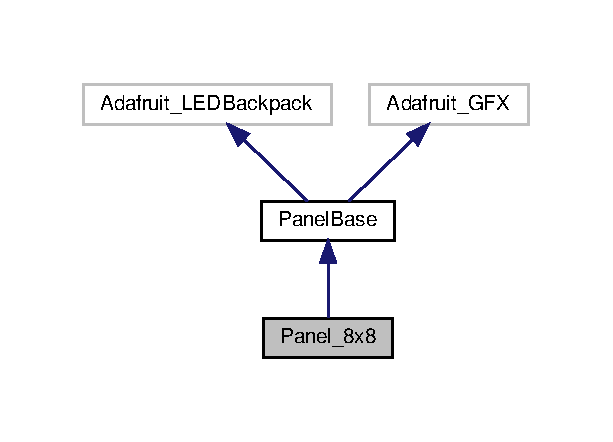
\includegraphics[width=294pt]{classPanel__8x8__inherit__graph}
\end{center}
\end{figure}


Collaboration diagram for Panel\+\_\+8x8\+:
\nopagebreak
\begin{figure}[H]
\begin{center}
\leavevmode
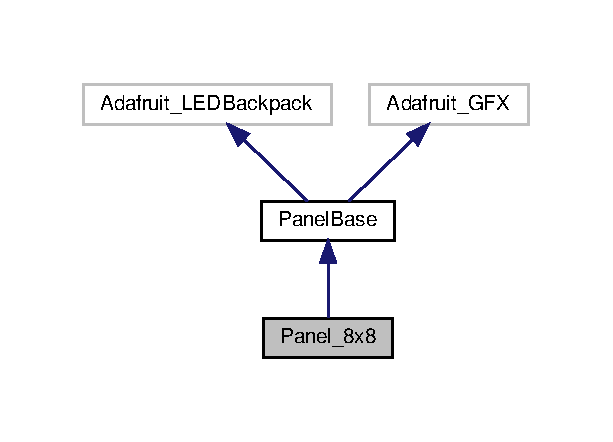
\includegraphics[width=294pt]{classPanel__8x8__coll__graph}
\end{center}
\end{figure}
\subsection*{Public Member Functions}
\begin{DoxyCompactItemize}
\item 
\mbox{\Hypertarget{classPanel__8x8_af52db8ce00f41e085ef8c45371fcb6db}\label{classPanel__8x8_af52db8ce00f41e085ef8c45371fcb6db}} 
\hyperlink{classPanel__8x8_af52db8ce00f41e085ef8c45371fcb6db}{Panel\+\_\+8x8} ()
\begin{DoxyCompactList}\small\item\em 8x8すべてが\+L\+E\+Dのパネルとして初期化 \end{DoxyCompactList}\end{DoxyCompactItemize}
\subsection*{Additional Inherited Members}


\subsection{Detailed Description}
8x8サイズの\+L\+E\+Dパネルクラス 

The documentation for this class was generated from the following files\+:\begin{DoxyCompactItemize}
\item 
src/\+Panel\+Manager/\hyperlink{Panel__8x8_8hpp}{Panel\+\_\+8x8.\+hpp}\item 
src/\+Panel\+Manager/Panel\+\_\+8x8.\+cpp\end{DoxyCompactItemize}

\hypertarget{classPanelBase}{}\section{Panel\+Base Class Reference}
\label{classPanelBase}\index{Panel\+Base@{Panel\+Base}}


1枚の\+L\+E\+Dパネルを表すクラス  




{\ttfamily \#include $<$Panel\+Base.\+hpp$>$}



Inheritance diagram for Panel\+Base\+:
\nopagebreak
\begin{figure}[H]
\begin{center}
\leavevmode
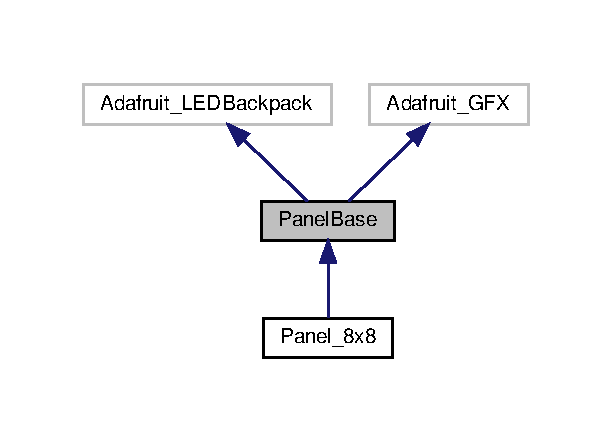
\includegraphics[width=294pt]{classPanelBase__inherit__graph}
\end{center}
\end{figure}


Collaboration diagram for Panel\+Base\+:
\nopagebreak
\begin{figure}[H]
\begin{center}
\leavevmode
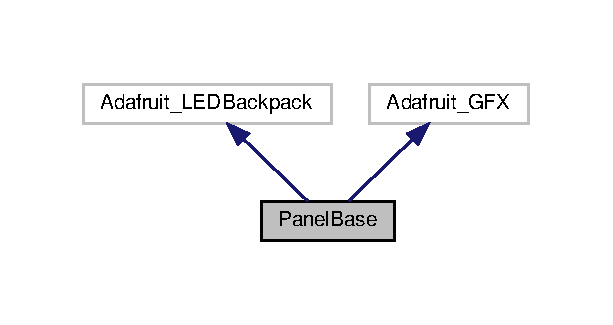
\includegraphics[width=294pt]{classPanelBase__coll__graph}
\end{center}
\end{figure}
\subsection*{Public Member Functions}
\begin{DoxyCompactItemize}
\item 
\mbox{\Hypertarget{classPanelBase_ae67aa479a006ead3f7ab01c6ce41e26b}\label{classPanelBase_ae67aa479a006ead3f7ab01c6ce41e26b}} 
\hyperlink{classPanelBase_ae67aa479a006ead3f7ab01c6ce41e26b}{Panel\+Base} (uint16\+\_\+t width=8, uint16\+\_\+t height=8)
\begin{DoxyCompactList}\small\item\em 矩形マトリクス\+L\+E\+D用コンストラクタ \end{DoxyCompactList}\item 
\mbox{\Hypertarget{classPanelBase_aece79bece96754da41945381d63a08fb}\label{classPanelBase_aece79bece96754da41945381d63a08fb}} 
void \hyperlink{classPanelBase_aece79bece96754da41945381d63a08fb}{update} ()
\begin{DoxyCompactList}\small\item\em メインループにて\+L\+E\+D全体の点灯状態を更新する \end{DoxyCompactList}\item 
\mbox{\Hypertarget{classPanelBase_a45f3a84f68861b3ae1bb34056bfd0d12}\label{classPanelBase_a45f3a84f68861b3ae1bb34056bfd0d12}} 
void \hyperlink{classPanelBase_a45f3a84f68861b3ae1bb34056bfd0d12}{draw\+Pixel} (int16\+\_\+t x, int16\+\_\+t y, uint16\+\_\+t color) override
\begin{DoxyCompactList}\small\item\em 指定座標を指定した色で点灯する(現状1bit) \end{DoxyCompactList}\end{DoxyCompactItemize}
\subsection*{Protected Member Functions}
\begin{DoxyCompactItemize}
\item 
\mbox{\Hypertarget{classPanelBase_a93b3be0e1305053c49d41e60e5bcd95c}\label{classPanelBase_a93b3be0e1305053c49d41e60e5bcd95c}} 
virtual void \hyperlink{classPanelBase_a93b3be0e1305053c49d41e60e5bcd95c}{register\+Matrix\+Info} ()=0
\begin{DoxyCompactList}\small\item\em マトリクスの各ピクセルの情報を登録する \end{DoxyCompactList}\item 
\mbox{\Hypertarget{classPanelBase_a4f9d7f1571a34a91574f078e5be49826}\label{classPanelBase_a4f9d7f1571a34a91574f078e5be49826}} 
int \hyperlink{classPanelBase_a4f9d7f1571a34a91574f078e5be49826}{calcX} (int x)
\begin{DoxyCompactList}\small\item\em 指定したいx座標を\+L\+E\+Dパネル上のx座標に変換する \end{DoxyCompactList}\item 
\mbox{\Hypertarget{classPanelBase_a0d128c31d63506c90d2d103a07ef5ac9}\label{classPanelBase_a0d128c31d63506c90d2d103a07ef5ac9}} 
int \hyperlink{classPanelBase_a0d128c31d63506c90d2d103a07ef5ac9}{calcY} (int y)
\begin{DoxyCompactList}\small\item\em 指定したいy座標を\+L\+E\+Dパネル上のy座標に変換する \end{DoxyCompactList}\end{DoxyCompactItemize}
\subsection*{Protected Attributes}
\begin{DoxyCompactItemize}
\item 
\mbox{\Hypertarget{classPanelBase_a2bd215863e490bf3d5e53f97ae1268fd}\label{classPanelBase_a2bd215863e490bf3d5e53f97ae1268fd}} 
std\+::vector$<$ \hyperlink{structPixelInfo}{Pixel\+Info} $>$ \hyperlink{classPanelBase_a2bd215863e490bf3d5e53f97ae1268fd}{pixels\+\_\+info\+\_\+}
\begin{DoxyCompactList}\small\item\em 各ピクセルの情報を格納する配列 \end{DoxyCompactList}\item 
\mbox{\Hypertarget{classPanelBase_a46af10a6ac5867c26b5ae13406f7c710}\label{classPanelBase_a46af10a6ac5867c26b5ae13406f7c710}} 
uint16\+\_\+t {\bfseries width\+\_\+}
\item 
\mbox{\Hypertarget{classPanelBase_a11f4802767a6e7954ff6e288cf94d21d}\label{classPanelBase_a11f4802767a6e7954ff6e288cf94d21d}} 
uint16\+\_\+t {\bfseries height\+\_\+}
\end{DoxyCompactItemize}


\subsection{Detailed Description}
1枚の\+L\+E\+Dパネルを表すクラス 

The documentation for this class was generated from the following files\+:\begin{DoxyCompactItemize}
\item 
src/\+Panel\+Manager/\hyperlink{PanelBase_8hpp}{Panel\+Base.\+hpp}\item 
src/\+Panel\+Manager/\hyperlink{PanelBase_8cpp}{Panel\+Base.\+cpp}\end{DoxyCompactItemize}

\hypertarget{structPixelInfo}{}\section{Pixel\+Info Struct Reference}
\label{structPixelInfo}\index{Pixel\+Info@{Pixel\+Info}}


各ピクセル情報を格納する構造体  




{\ttfamily \#include $<$Pixel\+Info.\+hpp$>$}

\subsection*{Public Member Functions}
\begin{DoxyCompactItemize}
\item 
\mbox{\Hypertarget{structPixelInfo_a1cfb39b0dd82a5bac358b0d7f2a6cc37}\label{structPixelInfo_a1cfb39b0dd82a5bac358b0d7f2a6cc37}} 
{\bfseries Pixel\+Info} (\hyperlink{PixelInfo_8hpp_a045ad070577d6987c818af7bc910ae1a}{E\+Chip\+Type} type, int color)
\end{DoxyCompactItemize}
\subsection*{Public Attributes}
\begin{DoxyCompactItemize}
\item 
\mbox{\Hypertarget{structPixelInfo_a3591ab17d9760da336e281c1e37682be}\label{structPixelInfo_a3591ab17d9760da336e281c1e37682be}} 
\hyperlink{PixelInfo_8hpp_a045ad070577d6987c818af7bc910ae1a}{E\+Chip\+Type} {\bfseries type\+\_\+}
\item 
\mbox{\Hypertarget{structPixelInfo_ac211b0b05b1e918bba9fdff7c09a347a}\label{structPixelInfo_ac211b0b05b1e918bba9fdff7c09a347a}} 
int {\bfseries color\+\_\+}
\end{DoxyCompactItemize}


\subsection{Detailed Description}
各ピクセル情報を格納する構造体 

The documentation for this struct was generated from the following files\+:\begin{DoxyCompactItemize}
\item 
src/\+Panel\+Manager/\hyperlink{PixelInfo_8hpp}{Pixel\+Info.\+hpp}\item 
src/\+Panel\+Manager/\hyperlink{PixelInfo_8cpp}{Pixel\+Info.\+cpp}\end{DoxyCompactItemize}

\chapter{File Documentation}
\hypertarget{Panel__8x8_8hpp}{}\section{src/\+Panel\+Manager/\+Panel\+\_\+8x8.hpp File Reference}
\label{Panel__8x8_8hpp}\index{src/\+Panel\+Manager/\+Panel\+\_\+8x8.\+hpp@{src/\+Panel\+Manager/\+Panel\+\_\+8x8.\+hpp}}


8x8サイズの\+L\+E\+Dパネルクラス  


{\ttfamily \#include \char`\"{}Panel\+Base.\+hpp\char`\"{}}\newline
Include dependency graph for Panel\+\_\+8x8.\+hpp\+:
\nopagebreak
\begin{figure}[H]
\begin{center}
\leavevmode
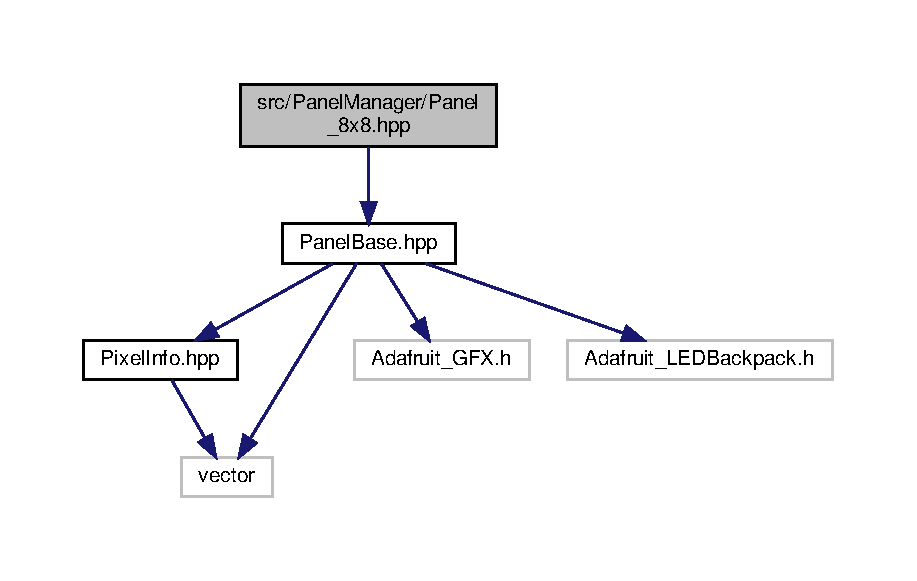
\includegraphics[width=350pt]{Panel__8x8_8hpp__incl}
\end{center}
\end{figure}
\subsection*{Classes}
\begin{DoxyCompactItemize}
\item 
class \hyperlink{classPanel__8x8}{Panel\+\_\+8x8}
\begin{DoxyCompactList}\small\item\em 8x8サイズの\+L\+E\+Dパネルクラス \end{DoxyCompactList}\end{DoxyCompactItemize}


\subsection{Detailed Description}
8x8サイズの\+L\+E\+Dパネルクラス 

\begin{DoxyAuthor}{Author}
Yoshito Nakaue 
\end{DoxyAuthor}
\begin{DoxyDate}{Date}
2021/07/11 
\end{DoxyDate}

\hypertarget{PanelBase_8cpp}{}\section{src/\+Panel\+Manager/\+Panel\+Base.cpp File Reference}
\label{PanelBase_8cpp}\index{src/\+Panel\+Manager/\+Panel\+Base.\+cpp@{src/\+Panel\+Manager/\+Panel\+Base.\+cpp}}


L\+E\+Dパネルの基底クラスの実装  


{\ttfamily \#include \char`\"{}Panel\+Base.\+hpp\char`\"{}}\newline
{\ttfamily \#include $<$utility$>$}\newline
Include dependency graph for Panel\+Base.\+cpp\+:
\nopagebreak
\begin{figure}[H]
\begin{center}
\leavevmode
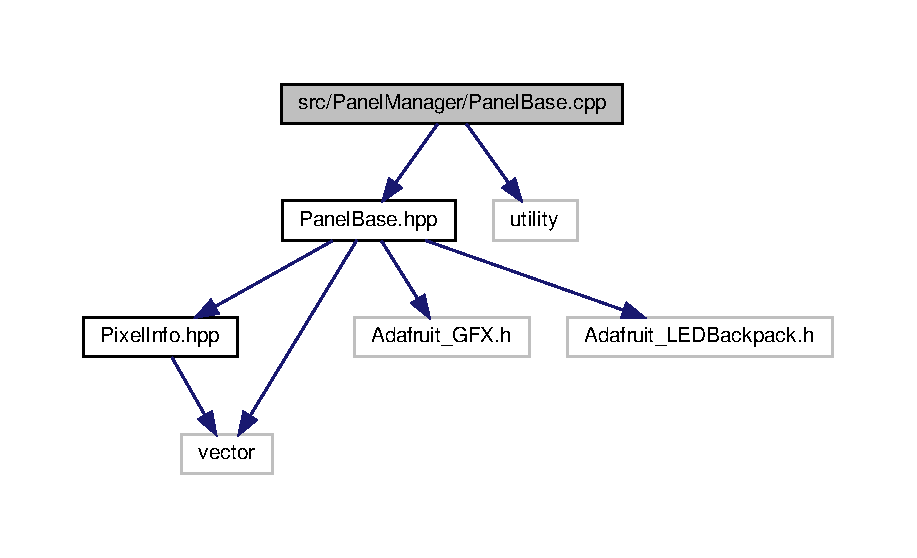
\includegraphics[width=350pt]{PanelBase_8cpp__incl}
\end{center}
\end{figure}


\subsection{Detailed Description}
L\+E\+Dパネルの基底クラスの実装 

\begin{DoxyAuthor}{Author}
Yoshito Nakaue 
\end{DoxyAuthor}
\begin{DoxyDate}{Date}
2021/07/05 
\end{DoxyDate}

\hypertarget{PanelBase_8hpp}{}\section{src/\+Panel\+Manager/\+Panel\+Base.hpp File Reference}
\label{PanelBase_8hpp}\index{src/\+Panel\+Manager/\+Panel\+Base.\+hpp@{src/\+Panel\+Manager/\+Panel\+Base.\+hpp}}


L\+E\+Dパネルの基底クラス  


{\ttfamily \#include \char`\"{}Pixel\+Info.\+hpp\char`\"{}}\newline
{\ttfamily \#include $<$vector$>$}\newline
{\ttfamily \#include $<$Adafruit\+\_\+\+G\+F\+X.\+h$>$}\newline
{\ttfamily \#include $<$Adafruit\+\_\+\+L\+E\+D\+Backpack.\+h$>$}\newline
Include dependency graph for Panel\+Base.\+hpp\+:
\nopagebreak
\begin{figure}[H]
\begin{center}
\leavevmode
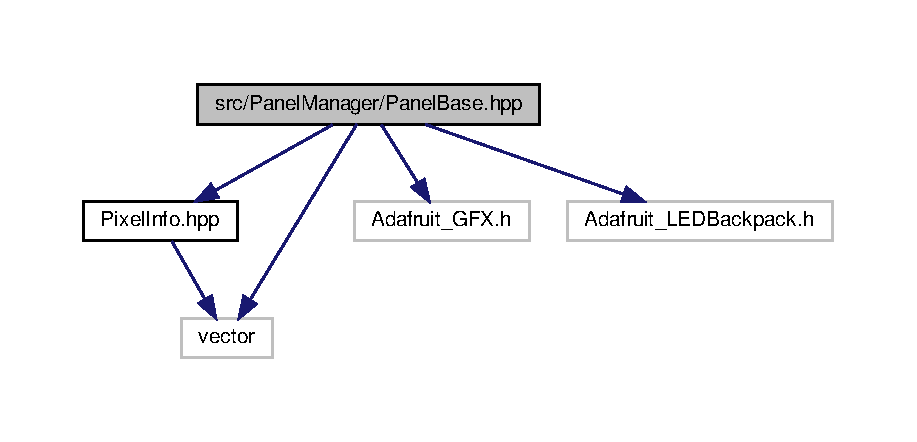
\includegraphics[width=350pt]{PanelBase_8hpp__incl}
\end{center}
\end{figure}
This graph shows which files directly or indirectly include this file\+:
\nopagebreak
\begin{figure}[H]
\begin{center}
\leavevmode
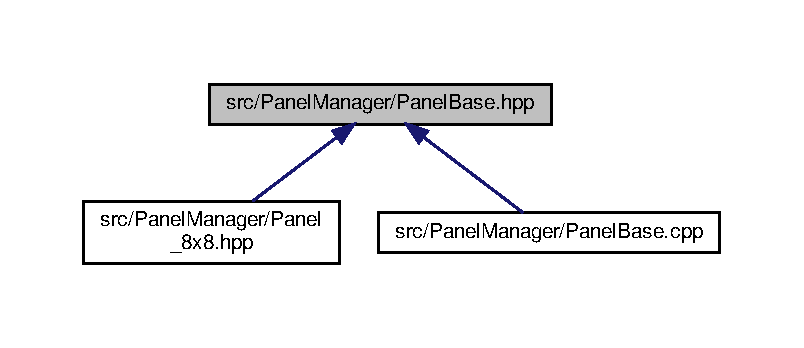
\includegraphics[width=244pt]{PanelBase_8hpp__dep__incl}
\end{center}
\end{figure}
\subsection*{Classes}
\begin{DoxyCompactItemize}
\item 
class \hyperlink{classPanelBase}{Panel\+Base}
\begin{DoxyCompactList}\small\item\em 1枚の\+L\+E\+Dパネルを表すクラス \end{DoxyCompactList}\end{DoxyCompactItemize}


\subsection{Detailed Description}
L\+E\+Dパネルの基底クラス 

\begin{DoxyAuthor}{Author}
Yoshito Nakaue 
\end{DoxyAuthor}
\begin{DoxyDate}{Date}
2021/07/05 
\end{DoxyDate}

\hypertarget{PixelInfo_8cpp}{}\section{src/\+Panel\+Manager/\+Pixel\+Info.cpp File Reference}
\label{PixelInfo_8cpp}\index{src/\+Panel\+Manager/\+Pixel\+Info.\+cpp@{src/\+Panel\+Manager/\+Pixel\+Info.\+cpp}}


各ピクセルの情報を格納する構造体の実装  


{\ttfamily \#include \char`\"{}Pixel\+Info.\+hpp\char`\"{}}\newline
Include dependency graph for Pixel\+Info.\+cpp\+:\nopagebreak
\begin{figure}[H]
\begin{center}
\leavevmode
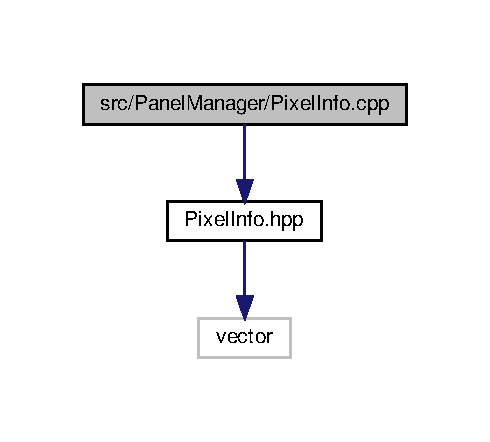
\includegraphics[width=235pt]{PixelInfo_8cpp__incl}
\end{center}
\end{figure}


\subsection{Detailed Description}
各ピクセルの情報を格納する構造体の実装 

\begin{DoxyAuthor}{Author}
Yoshito Nakaue 
\end{DoxyAuthor}
\begin{DoxyDate}{Date}
2021/07/09 
\end{DoxyDate}

\hypertarget{PixelInfo_8hpp}{}\section{src/\+Panel\+Manager/\+Pixel\+Info.hpp File Reference}
\label{PixelInfo_8hpp}\index{src/\+Panel\+Manager/\+Pixel\+Info.\+hpp@{src/\+Panel\+Manager/\+Pixel\+Info.\+hpp}}


各ピクセルの情報を格納する構造体を定義  


{\ttfamily \#include $<$vector$>$}\newline
Include dependency graph for Pixel\+Info.\+hpp\+:
\nopagebreak
\begin{figure}[H]
\begin{center}
\leavevmode
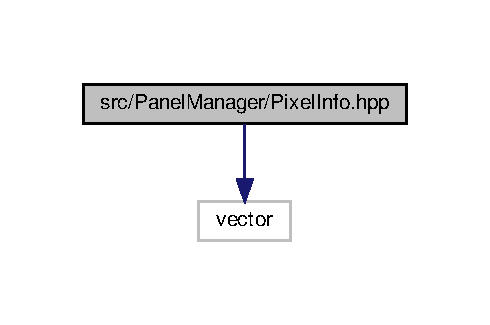
\includegraphics[width=235pt]{PixelInfo_8hpp__incl}
\end{center}
\end{figure}
This graph shows which files directly or indirectly include this file\+:
\nopagebreak
\begin{figure}[H]
\begin{center}
\leavevmode
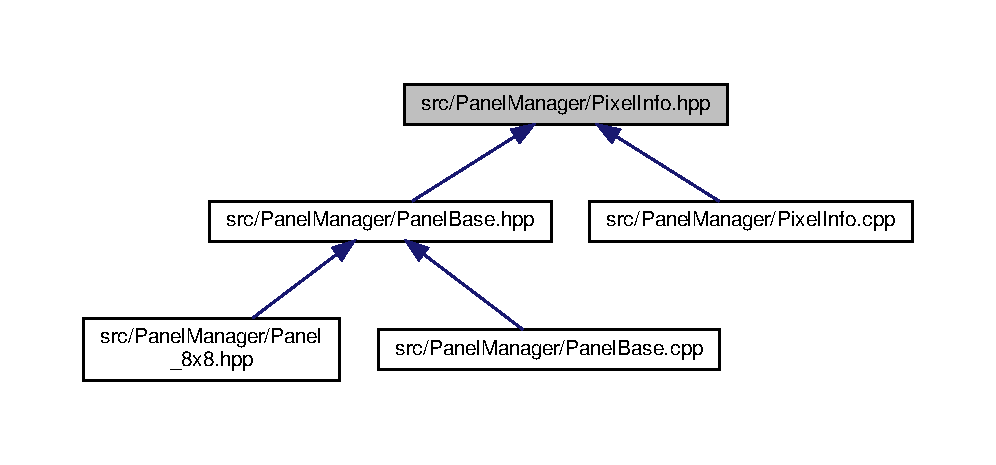
\includegraphics[width=350pt]{PixelInfo_8hpp__dep__incl}
\end{center}
\end{figure}
\subsection*{Classes}
\begin{DoxyCompactItemize}
\item 
struct \hyperlink{structPixelInfo}{Pixel\+Info}
\begin{DoxyCompactList}\small\item\em 各ピクセル情報を格納する構造体 \end{DoxyCompactList}\end{DoxyCompactItemize}
\subsection*{Enumerations}
\begin{DoxyCompactItemize}
\item 
\mbox{\Hypertarget{PixelInfo_8hpp_a045ad070577d6987c818af7bc910ae1a}\label{PixelInfo_8hpp_a045ad070577d6987c818af7bc910ae1a}} 
enum \hyperlink{PixelInfo_8hpp_a045ad070577d6987c818af7bc910ae1a}{E\+Chip\+Type} \+: uint8\+\_\+t \{ {\bfseries N\+O\+NE}, 
{\bfseries L\+ED}, 
{\bfseries I\+R\+\_\+\+L\+ED}, 
{\bfseries I\+R\+\_\+\+R\+CV}
 \}\begin{DoxyCompactList}\small\item\em L\+E\+D、赤外線センサ等の列挙型 \end{DoxyCompactList}
\end{DoxyCompactItemize}


\subsection{Detailed Description}
各ピクセルの情報を格納する構造体を定義 

\begin{DoxyAuthor}{Author}
Yoshito Nakaue 
\end{DoxyAuthor}
\begin{DoxyDate}{Date}
2021/07/07 
\end{DoxyDate}

%--- End generated contents ---

% Index
\backmatter
\newpage
\phantomsection
\clearemptydoublepage
\addcontentsline{toc}{chapter}{Index}
\printindex

\end{document}
